\documentclass[a4paper]{article}

%use the english line for english reports
%usepackage[english]{babel}
\usepackage[portuguese]{babel}
\usepackage[utf8]{inputenc}
\usepackage{indentfirst}
\usepackage{graphicx}
\usepackage{verbatim}
\usepackage{alltt}
\renewcommand{\ttdefault}{txtt}


\begin{document}

\setlength{\textwidth}{16cm}
\setlength{\textheight}{22cm}

\title{\Huge\textbf{Q!nto}\linebreak\linebreak\linebreak
\Large\textbf{Relatório Intercalar}\linebreak\linebreak
\linebreak\linebreak

\includegraphics[scale=0.1]{feup-logo.png}\linebreak\linebreak
\linebreak\linebreak
\Large{Mestrado Integrado em Engenharia Informática e Computação} \linebreak\linebreak
\Large{Programação em Lógica}\linebreak
}

\author{\textbf{Grupo 2:}\\
Filipa Marilia Monteiro Ramos - up201305378 \\
Inês Alexandra dos Santos Carneiro - up201303501 \\
\linebreak\linebreak \\
 \\ Faculdade de Engenharia da Universidade do Porto \\ Rua Roberto Frias, s\/n, 4200-465 Porto, Portugal \linebreak\linebreak\linebreak
\linebreak\linebreak\vspace{1cm}}

\maketitle
\thispagestyle{empty}

%************************************************************************************************
%************************************************************************************************

\newpage

%Todas as figuras devem ser referidas no texto. %\ref{fig:codigoFigura}
%
%%Exemplo de código para inserção de figuras
%%\begin{figure}[h!]
%%\begin{center}
%%escolher entre uma das seguintes três linhas:
%%\includegraphics[height=20cm,width=15cm]{path relativo da imagem}
%%\includegraphics[scale=0.5]{path relativo da imagem}
%%\includegraphics{path relativo da imagem}
%%\caption{legenda da figura}
%%\label{fig:codigoFigura}
%%\end{center}
%%\end{figure}
%
%
%\textit{Para escrever em itálico}
%\textbf{Para escrever em negrito}
%Para escrever em letra normal
%``Para escrever texto entre aspas''
%
%Para fazer parágrafo, deixar uma linha em branco.
%
%Como fazer bullet points:
%\begin{itemize}
	%\item Item1
	%\item Item2
%\end{itemize}
%
%Como enumerar itens:
%\begin{enumerate}
	%\item Item 1
	%\item Item 2
%\end{enumerate}
%
%\begin{quote}``Isto é uma citação''\end{quote}


%%%%%%%%%%%%%%%%%%%%%%%%%%
\section{O Jogo Q!nto}

\begin{figure}[ht!]
\centering
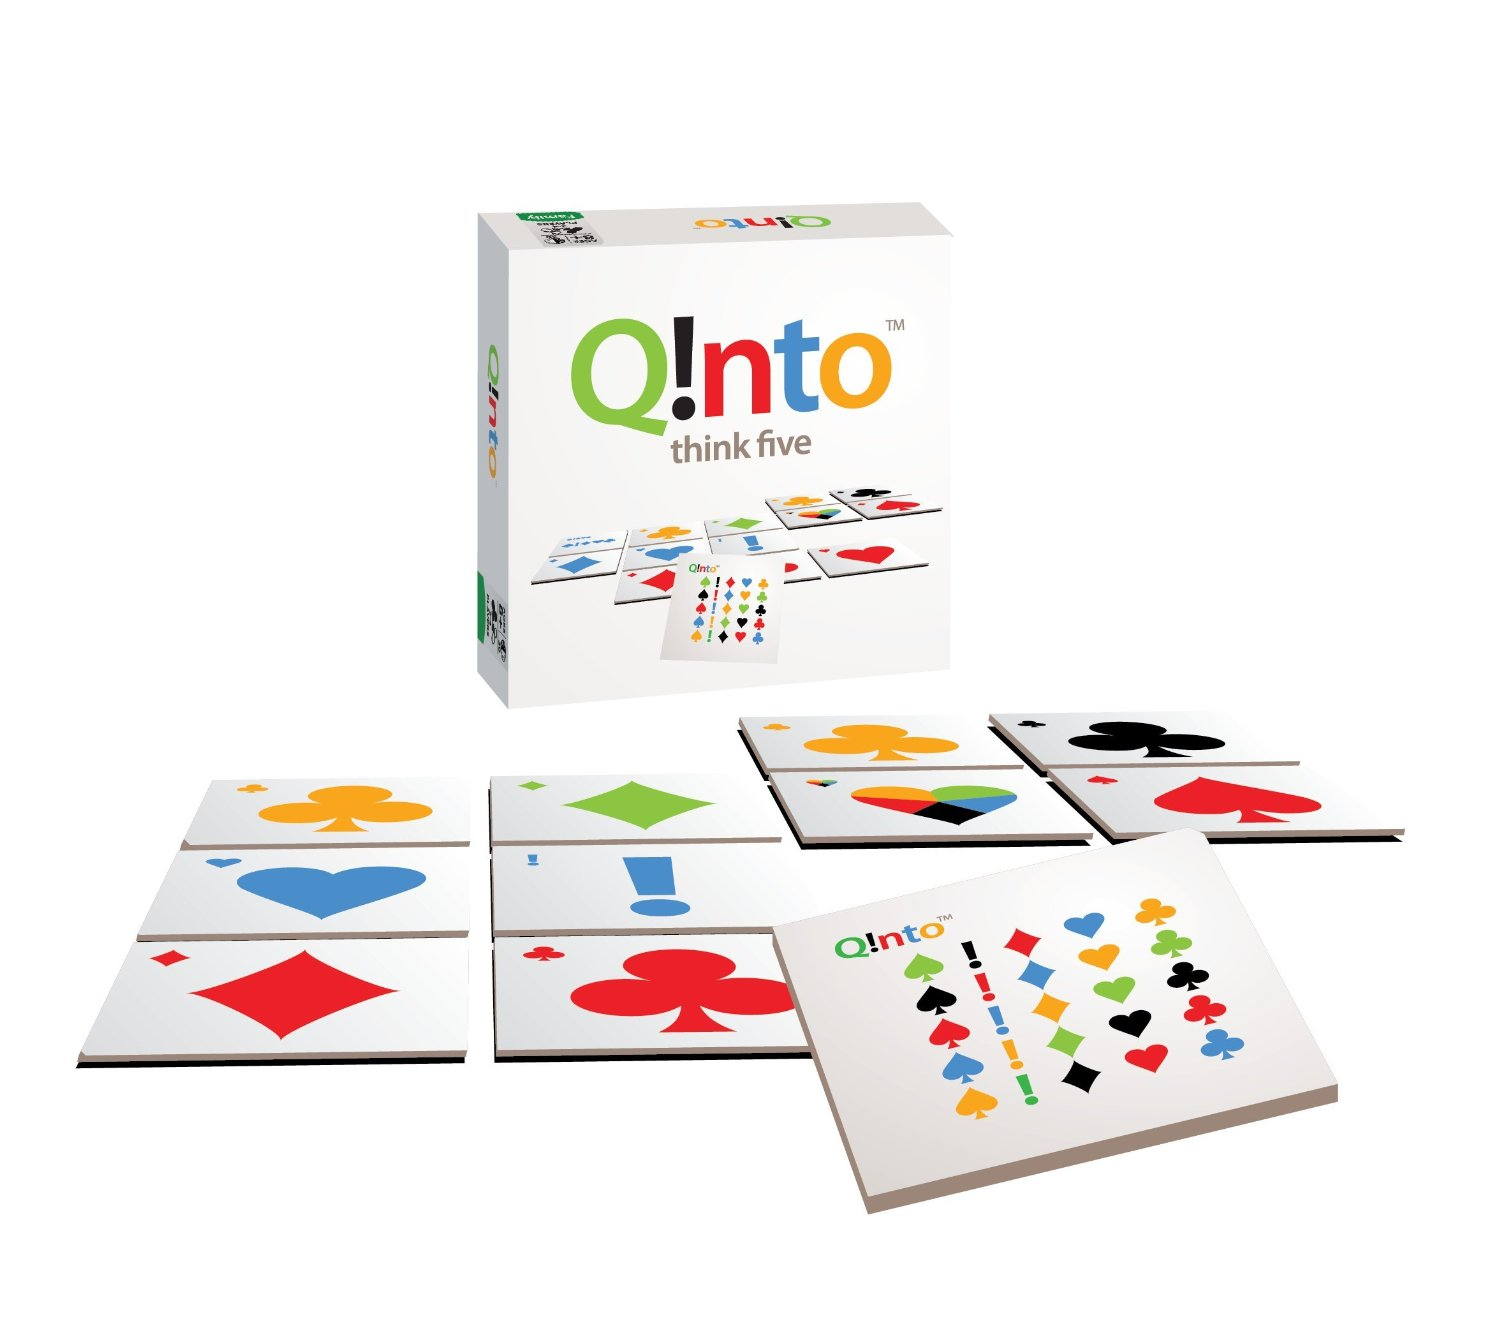
\includegraphics[width=90mm]{q!ntologo.jpg}
\caption{Caixa e cartas do jog. \label{q!nto}}
\end{figure}

\subsection{História}

Q!nto é um jogo de estratégia abstrata que foi desenvolvido pelo designer Gene Mackles e publicado pela PDG games. O seu lançamento no mercado data do ano 2014. É adequado para todas as idades a partir dos 8 anos podendo ser jogado por um mínimo de 2 e um máximo de 4 jogadores. Existem 3 variações de Q!nto: Q!nto clássico que será o desenvolvido pelo grupo; Q!nto Plus que permite a contagem de pontos numa diagonal de 3 ou mais cartas e Q!nto Light no qual as cartas são divididas igualmente pelos jogadores e o vencedor é o que esvazia a sua mão primeiro. 

\subsection{Regras}

Cada jogador possui 5 cartas sendo que existem 5 formas e 5 cores possíveis. Existem cartas, em menor número, que permitem escolher ou a sua forma ou a sua cor ou ambas.

\begin{enumerate}
	\item Carta que permite escolher a cor: tem uma forma específica e o utilizador escolhe a cor que esta possuí. 
	\item Carta que permite escolher a forma: tem uma cor definida e permite a escolha da forma da mesma.
	\item Carta universal: forma e cor definível. 
\end{enumerate}

\par
Uma jogada é válida se for feita uma coluna ou linha com cartas nas seguintes condições:

\begin{enumerate}
	\item símbolos iguais;
	\item cores iguais;
	\item símbolos e cores diferentes.
\end{enumerate}

\begin{figure}[ht!]
\centering

\includegraphics[width=65mm]{especiais.jpg}
\caption{Carta que permite escolher a cor, forma e universal. (1,2 e 3 respetivamente). \label{especiais}}
\end{figure}

\par
A pontuação é calculada com base no número de cartas por linha e coluna englobada na jogada. A cada carta é dada a pontuação de uma unidade. A mesma carta pode ser contabilizada duas vezes visto que os pontos são cotados horizontal e verticalmente. Quando se obtêm linhas com 5 elementos o jogador recebe uma pontuação extra de 5 pontos. Esta jogada é apelidada de Q!nto. Também se obtém 5 pontos extra quando são jogadas todas as cartas na mão e quando é a última jogada. O jogo acaba quando não existem mais cartas a serem jogadas e não existem cartas na pilha. Ganha o jogador com mais pontos.

\begin{figure}[h]
\centering
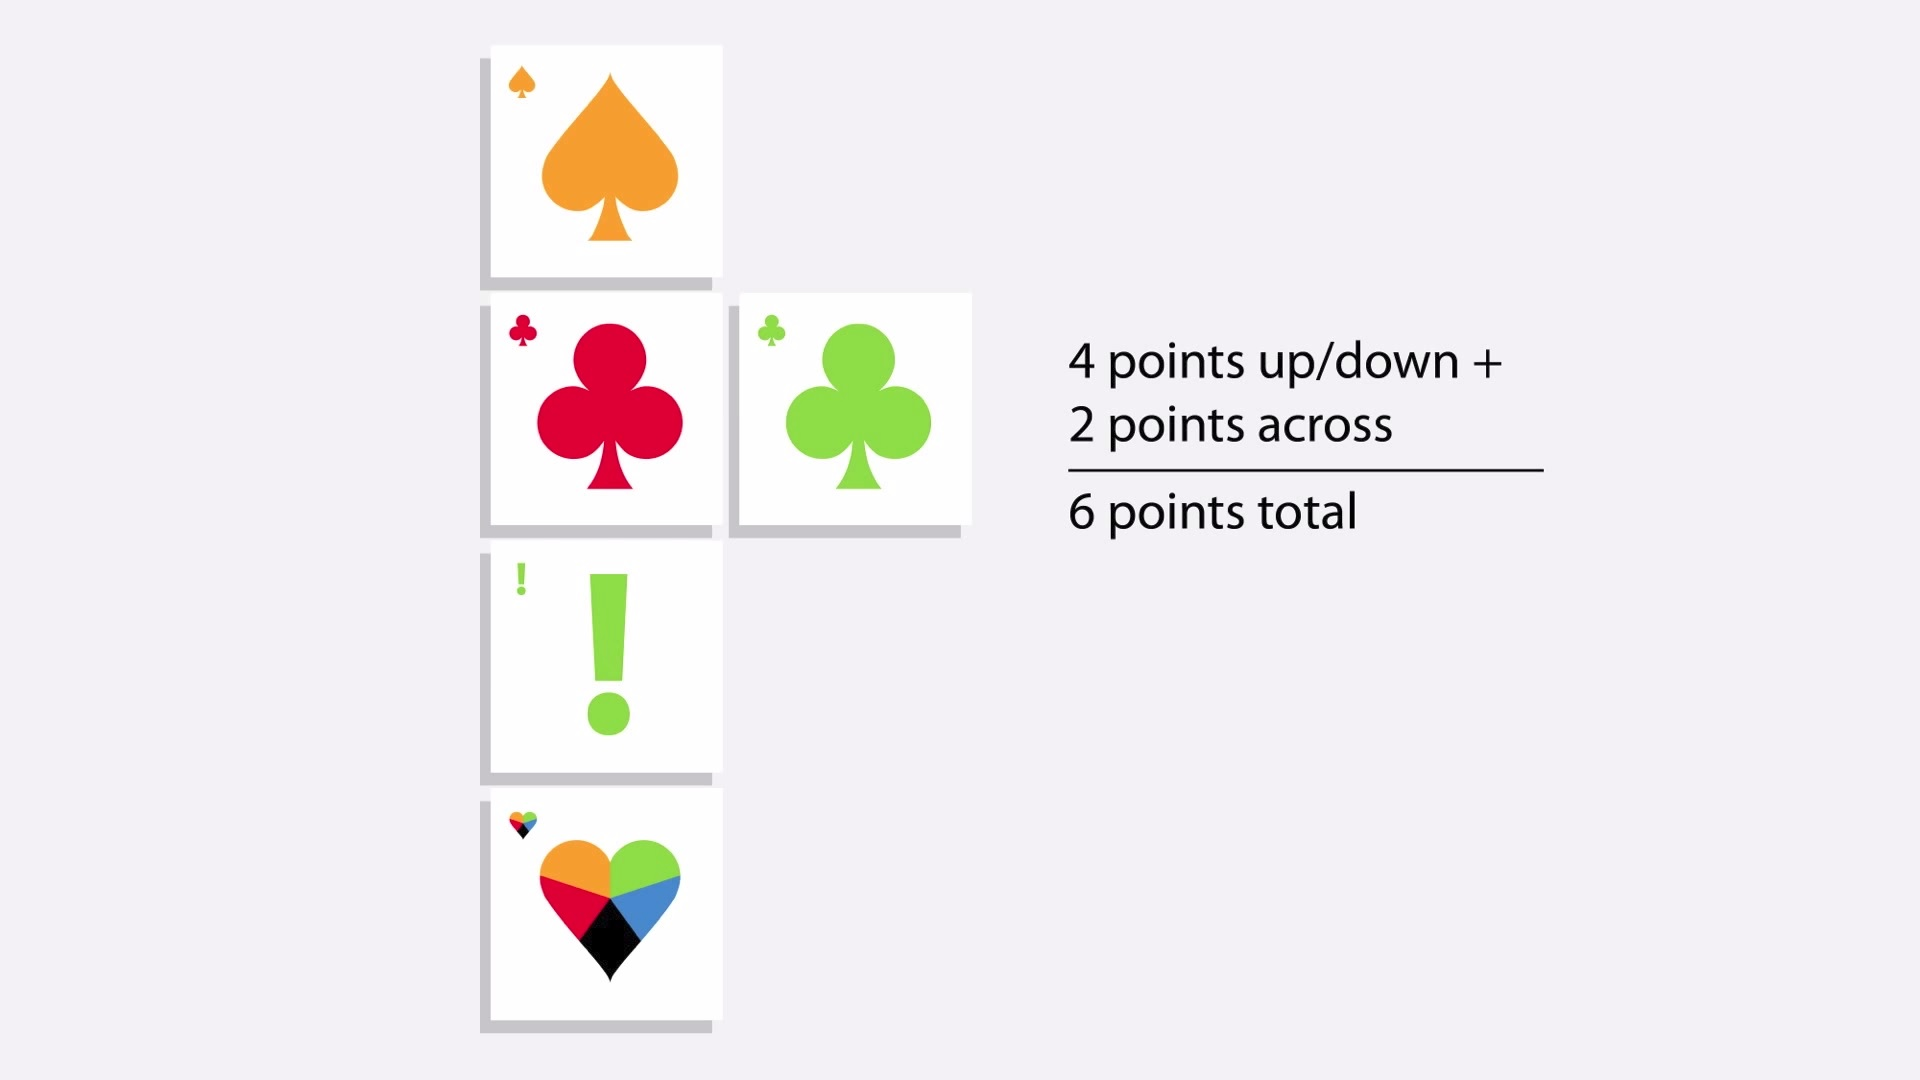
\includegraphics[width=80mm]{points.jpg}
\caption{Contagem dos pontos. \label{points1}}
\end{figure}

\begin{figure}[hb!]
\centering
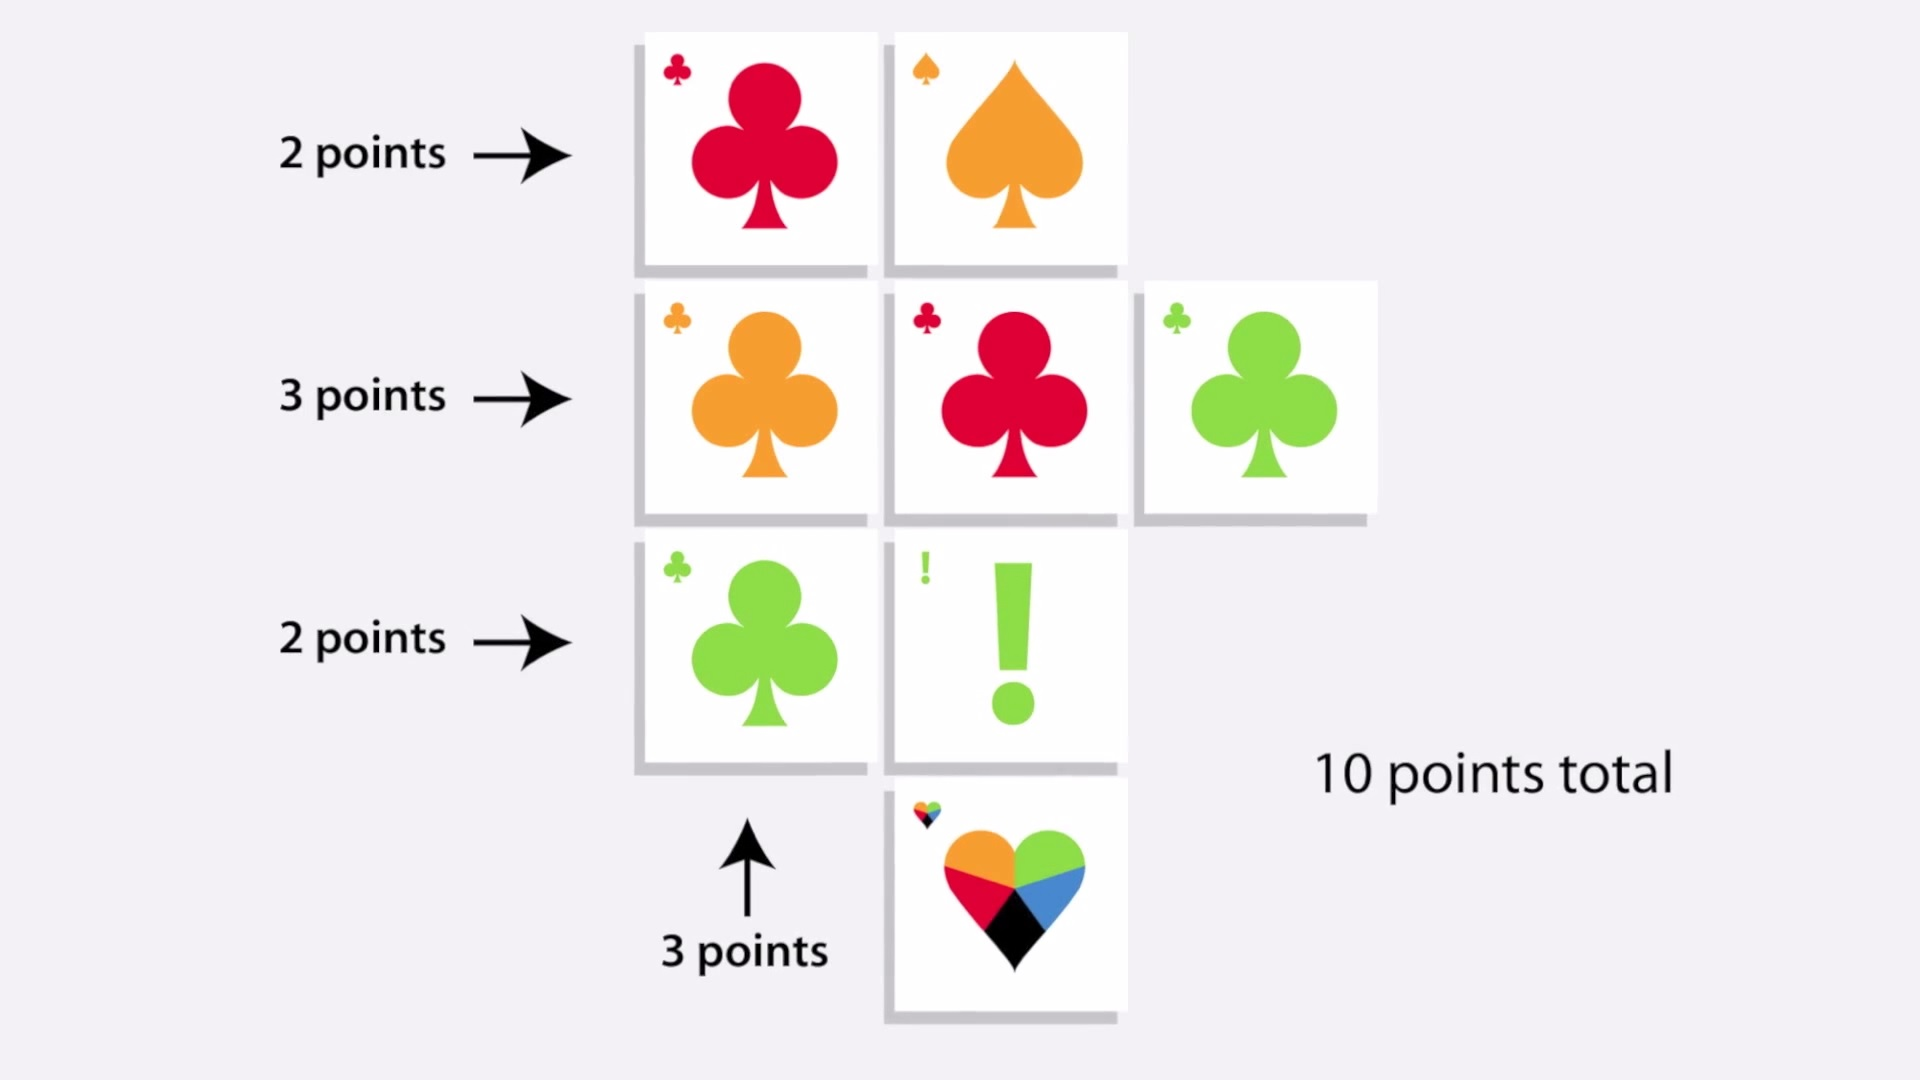
\includegraphics[width=80mm]{points2.jpg}
\caption{Contagem dos pontos (exemplo 2). \label{points2}}
\end{figure}

\begin{figure}[ht!]
\centering
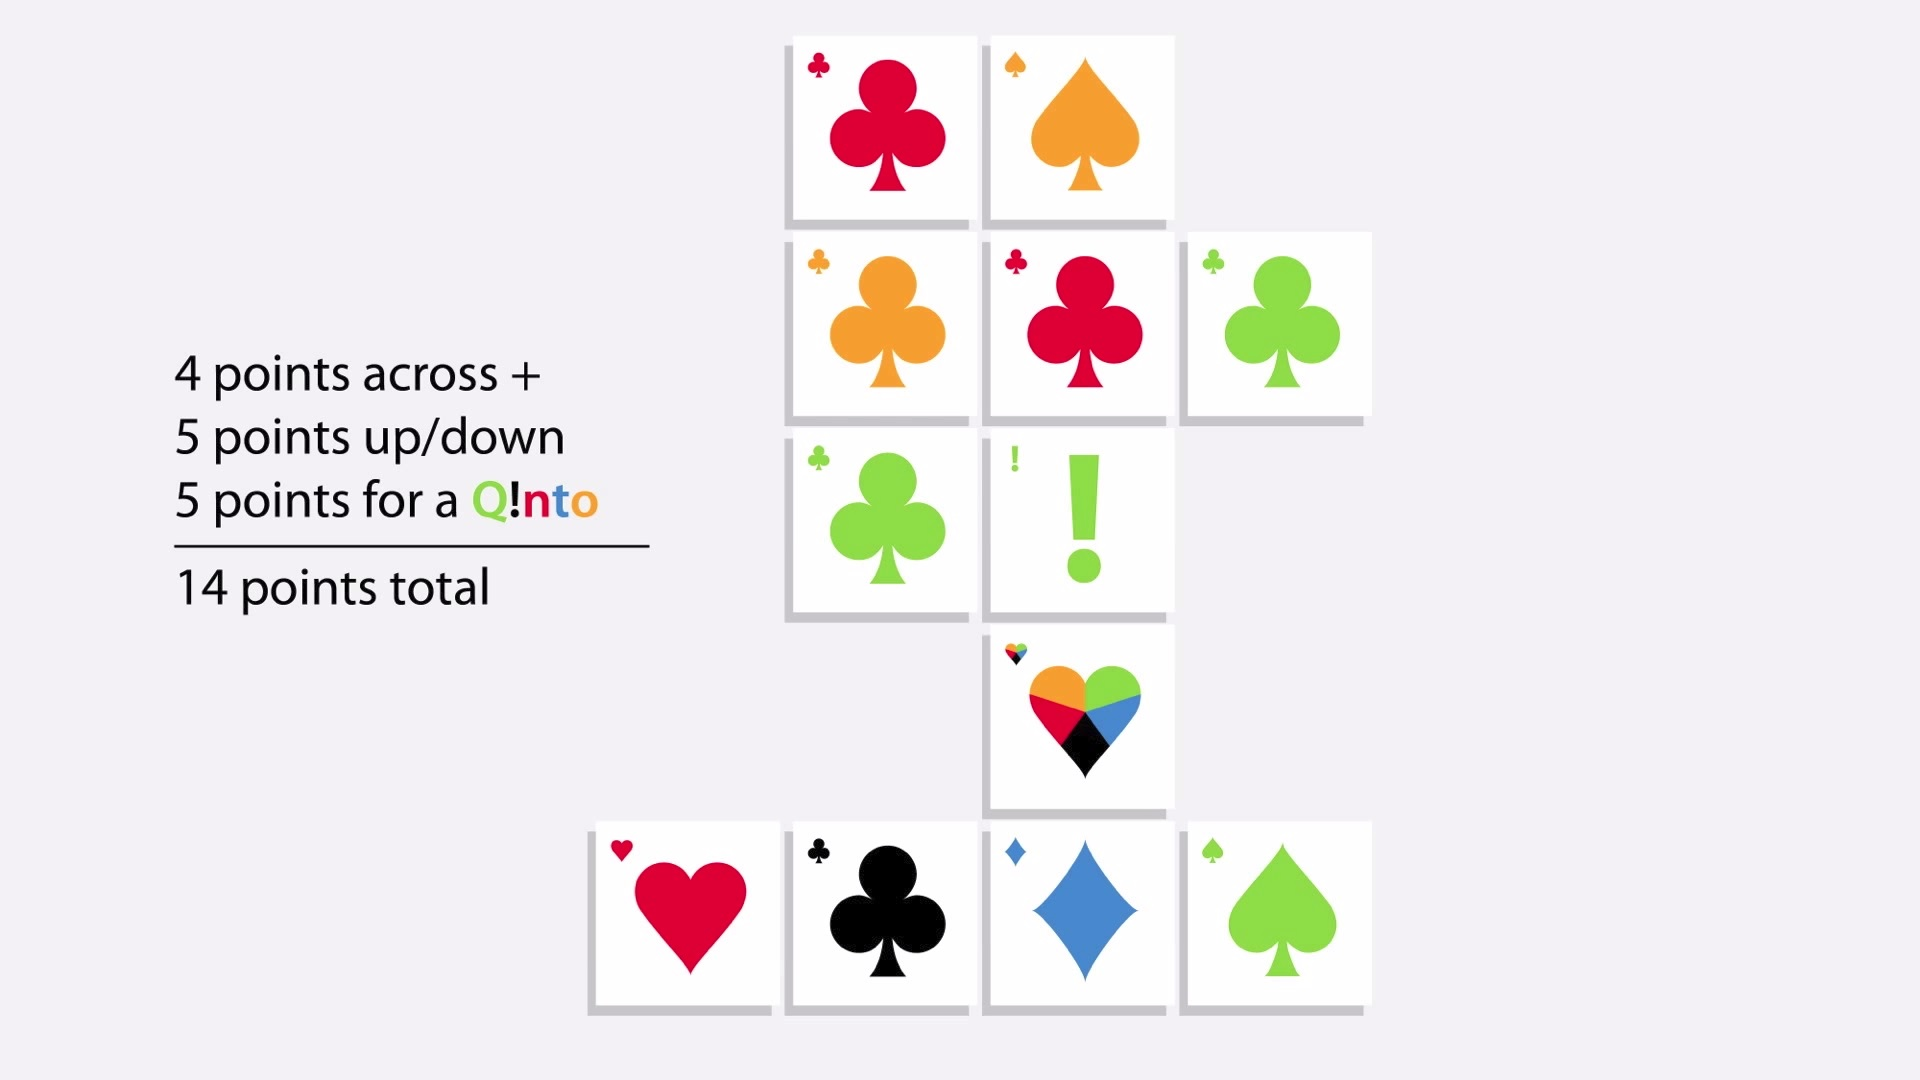
\includegraphics[width=80mm]{quinto.jpg}
\caption{Jogada Q!into. \label{quinto}}
\end{figure}

%%%%%%%%%%%%%%%%%%%%%%%%%%
\section{Representação do Estado do Jogo}

O menu inicial permitirá a escolha entre as seguintes possibilidades:

\begin{enumerate}
	\item Jogador vs Jogador;
	\item Jogador vs Computador;
	\item Computador vs Computador;
	\item Sair do Jogo. 
\end{enumerate}

\par
O tabuleiro inicial corresponde a uma grelha de 5x5. À medida que o jogo evolui, o tabuleiro é aumentado 5 casas horizontal e verticalmente. Inicialmente, o tabuleiro tem apenas uma carta no centro que é escolhida de forma aleatória da pilha. Por baixo do tabuleiro é representada a mão do jogador (5 cartas). A cada jogada é atualizado o tabuleiro posicionando as cartas jogadas e são dadas cartas a quem as gastou de modo a perfazer 5. O estado de vitória ou derrota corresponde ao final do jogo e é identificada através de uma mensagem no ecrã.

%%%%%%%%%%%%%%%%%%%%%%%%%%
\section{Visualização do Tabuleiro}

A representação do tabuleiro será feita de forma textual através de barras e \textit{underscores}.

\begin{figure}[h!]
\centering
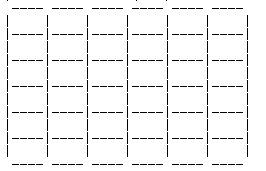
\includegraphics[width=50mm]{board.jpg}
\caption{Tabuleiro exemplo visualizado no SICStus de 6x6. \label{board}}
\end{figure}

Os predicados implementados foram os seguintes:

\begin{alltt}
	fguideLine(N, CC) :- CC==N, write('    ').
	fguideLine(N, CC) :- CC < N, CC2 is CC+1, write('    '), \newline L is 65+CC, format('~1c', [L]) , write(' '), fguideLine(N, CC2).
\end{alltt}
		\normalfont - escreve os números das linhas e as letras identificadoras das colunas.
\begin{alltt}
	fHorizontalLine(0).
	fHorizontalLine(N) :- N>0 , write('  '), write('----'), N1 is N-1,\newline fHorizontalLine(N1).

		 \normalfont - f significa "first", ou seja, os predicados com f desenham a primeira linha do tabuleiro.
\end{alltt}
\begin{alltt}
	sHorizontalLine(0, [], \_CC) :- write('|'),write(' '), write(\_CC).
	sHorizontalLine(N, [L|R], \_CC) :- N>0 , write(\_CC), write(' '), \newline write('|'), writetile(L), N1 is N-1, sHorizontalLine(N1, R, \_CC2).
\end{alltt}
		\normalfont  - s significa "second", ou seja, estes predicados desenham a "segunda" linha do tabuleiro o que corresponde a todas as linhas entre a primeira e a última.

\begin{alltt}
	tHorizontalLine(0) :-  write('|').
	tHorizontalLine(N) :- N>0, write(' '), write('|'), \newline write('----'), N1 is N-1 , tHorizontalLine(N1).
\end{alltt}
		\normalfont - t refere-se a "third" sendo estes os predicados que desenham a última linha do tabuleiro.

\begin{alltt}
	displayBoardaux([]).
	displayBoardaux([L1]) :- length(L1,N1), sHorizontalLine(N1,L1,0), nl.
	displayBoardaux([L1|R]) :- R \= [], length(L1,N1),  \newline sHorizontalLine(N1, L1,0), nl, tHorizontalLine(N1), nl, displayBoardaux(R).
\end{alltt}
		\normalfont - predicados auxiliares que ajudam a fazer o display do tabuleiro.

\begin{alltt}
	listElement([],0, _X).
	listElement([X|Xs], N, X) :- N1 is N - 1,  listElement(Xs, N1, X).
\end{alltt}
		\normalfont - mais predicados que auxiliam na construção do tabuleiro. 
\begin{alltt}
	displayBoard([L1|R]) :-  length(L1,N1), nl, fguideLine(N1, 0), nl, \newline fHorizontalLine(N1), nl, displayBoardaux([L1|R]), \newline fHorizontalLine(N1), nl, fguideLine(N1, 0), nl.
\end{alltt}
		\normalfont - predicado que faz o display do tabuleiro.

\begin{alltt}
	createMatrix(W, H, Matrix) :- listElement(L,W,tile(' ',' ')), \newline listElement(Matrix,H,L). 
\end{alltt}
		\normalfont - cria a matriz que corresponde ao tabuleiro.

\begin{alltt}
	createBoard(W,H) :- createMatrix(W,H, B), displayBoard(B).
\end{alltt}
		\normalfont - faz output do tabuleiro e cria a matrix correspondente.
\begin{alltt}
	expand_matrix_up(Matrix, [L|Matrix]) :- empty_tile( E ), \newline matrix_width(Matrix, W), listElement(L, W, E).
	expand_matrix_down(Matrix, NewMatrix) :- empty_tile( E ), \newline matrix_width(Matrix, W), listElement(L, W, E),\newline append(Matrix, [L], NewMatrix).

	expand_matrix_left([],[]).
	expand_matrix_left([L|Matrix], [NL|NewMatrix]):- empty_tile( E ), \newline append([E], L, NL), expand_matrix_left(Matrix, NewMatrix).
	expand_matrix_right([],[]).
	expand_matrix_right([L|Matrix], [NL|NewMatrix]):- empty_tile( E ), \newline append(L, [E], NL), expand_matrix_right(Matrix, NewMatrix). 
\end{alltt}
		\normalfont - para expandir a matriz a cada jogada. 


%%%%%%%%%%%%%%%%%%%%%%%%%%
\section{Movimentos}

Os movimentos possíveis são em linha tanto horizontal como vertical. 

\section{Bibliografia}

\begin{enumerate}
	\item http://www.pdggames.com/images/resources/TriplePlayRulesmore.pdf
	\item http://www.pdggames.com/product/qnto
	\item https://www.youtube.com/watch?v=t0RolluapXg
	\item https://boardgamegeek.com/boardgame/164972/qnto
\end{enumerate}

\end{document}